\documentclass{article}\usepackage[]{graphicx}\usepackage[]{color}
% maxwidth is the original width if it is less than linewidth
% otherwise use linewidth (to make sure the graphics do not exceed the margin)
\makeatletter
\def\maxwidth{ %
  \ifdim\Gin@nat@width>\linewidth
    \linewidth
  \else
    \Gin@nat@width
  \fi
}
\makeatother

\definecolor{fgcolor}{rgb}{0.345, 0.345, 0.345}
\newcommand{\hlnum}[1]{\textcolor[rgb]{0.686,0.059,0.569}{#1}}%
\newcommand{\hlstr}[1]{\textcolor[rgb]{0.192,0.494,0.8}{#1}}%
\newcommand{\hlcom}[1]{\textcolor[rgb]{0.678,0.584,0.686}{\textit{#1}}}%
\newcommand{\hlopt}[1]{\textcolor[rgb]{0,0,0}{#1}}%
\newcommand{\hlstd}[1]{\textcolor[rgb]{0.345,0.345,0.345}{#1}}%
\newcommand{\hlkwa}[1]{\textcolor[rgb]{0.161,0.373,0.58}{\textbf{#1}}}%
\newcommand{\hlkwb}[1]{\textcolor[rgb]{0.69,0.353,0.396}{#1}}%
\newcommand{\hlkwc}[1]{\textcolor[rgb]{0.333,0.667,0.333}{#1}}%
\newcommand{\hlkwd}[1]{\textcolor[rgb]{0.737,0.353,0.396}{\textbf{#1}}}%
\let\hlipl\hlkwb

\usepackage{framed}
\makeatletter
\newenvironment{kframe}{%
 \def\at@end@of@kframe{}%
 \ifinner\ifhmode%
  \def\at@end@of@kframe{\end{minipage}}%
  \begin{minipage}{\columnwidth}%
 \fi\fi%
 \def\FrameCommand##1{\hskip\@totalleftmargin \hskip-\fboxsep
 \colorbox{shadecolor}{##1}\hskip-\fboxsep
     % There is no \\@totalrightmargin, so:
     \hskip-\linewidth \hskip-\@totalleftmargin \hskip\columnwidth}%
 \MakeFramed {\advance\hsize-\width
   \@totalleftmargin\z@ \linewidth\hsize
   \@setminipage}}%
 {\par\unskip\endMakeFramed%
 \at@end@of@kframe}
\makeatother

\definecolor{shadecolor}{rgb}{.97, .97, .97}
\definecolor{messagecolor}{rgb}{0, 0, 0}
\definecolor{warningcolor}{rgb}{1, 0, 1}
\definecolor{errorcolor}{rgb}{1, 0, 0}
\newenvironment{knitrout}{}{} % an empty environment to be redefined in TeX

\usepackage{alltt}
\usepackage{geometry}
\geometry{a4paper, margin=0.75in}
\usepackage{amsmath,amsthm,amssymb}
\usepackage{bm}
\usepackage{graphicx}
\usepackage[dvipsnames]{xcolor}
\usepackage{multicol}
\usepackage{multirow}
\usepackage{float}
\usepackage{siunitx}
\usepackage{xr}
\externaldocument[sup:]{supplement}
\usepackage[hidelinks]{hyperref}
\usepackage{cleveref}
\usepackage{authblk}
\usepackage{booktabs}
\usepackage{array}
\usepackage{colortbl}
\usepackage[]{caption}
\sisetup{output-exponent-marker=\ensuremath{\mathrm{e}}}

\renewcommand\Authfont{\small}
\renewcommand\Affilfont{\footnotesize}
\title{Pre-capture multiplexing provides additional power to detect copy number variation in exome sequencing}
\author[1,2]{Dayne L Filer}
\author[2]{Fengshen Kuo}
\author[1]{Alicia T Brandt}
\author[1]{Christian R Tilley}
\author[1]{Piotr A Mieczkowski}
\author[1,2,3]{Kimberly Robasky}
\author[2]{Chris Bizon}
\author[2]{Jeffery L Tilson}
\author[1,2]{Bradford C Powell}
\author[1,2]{Darius M Bost}
\author[1]{Clark D Jeffries}
\author[1]{Jonathan S Berg}
\author[1,2,4]{Kirk C Wilhelmsen}
\affil[1]{UNC School of Medicine, Department of Genetics, Chapel Hill, NC}
\affil[2]{Renaissance Computing Institute, Chapel Hill, NC}
\affil[3]{UNC School of Information and Library Science, Chapel Hill, NC}
\affil[4]{UNC School of Medicine, Department of Neurology, Chapel Hill, NC}
\date{}

%% Keep package name from getting hyphenated
\hyphenation{mcCNV}

\setlength{\parindent}{0em}
\setlength{\parskip}{1ex}
\IfFileExists{upquote.sty}{\usepackage{upquote}}{}
\begin{document}



\maketitle

%%----------------------------------------------------------------------------%%
%% Abstract
%%----------------------------------------------------------------------------%%

\begin{abstract}
\noindent\textbf{Motivation:}As exome sequencing (ES) integrates into clinical practice, we should make every effort to utilize all information generated.
Copy-number variation can lead to Mendelian disorders, but small copy-number variants (CNVs) often get overlooked or obscured by under-powered data collection.
Many groups have developed methodology for detecting copy-number variants from ES, but existing methods often perform poorly for small CNVs and rely on large sample numbers not always available to clinical laboratories.
Furthermore, methods often rely on Bayesian approaches requiring user-defined priors in the setting of insufficient prior knowledge.
\newline
\textbf{Results:}
We demonstrate: (1) pooling samples prior to capture (multiplexed capture) reduces inter-sample variance; (2) a novel depth-based algorithm (mcCNV) for detecting CNVs from multiplexed-capture ES data.
We contrast our novel approach without defining a prior to the commonly-used ExomeDepth.
When compared to calls made from matched genome sequencing, we find the mcCNV algorithm performs comparably to ExomeDepth.
\newline
\textbf{Availability and Implementation:} mcCNV is implemented as an R package. \url{https://github.com/daynefiler/mcCNV}
\newline
\textbf{Contact:} Dayne Filer, \href{mailto:dayne_filer@med.unc.edu}{dayne\_filer@med.unc.edu}.
\newline
\textbf{Supplemental information:} All data and functionality to produce this manuscript provided in a standalone R package with a vignette replicating the analysis. \url{https://github.com/daynefiler/filer2020A}
\end{abstract}

%%----------------------------------------------------------------------------%%
%% Introduction
%%----------------------------------------------------------------------------%%

\section{Introduction}

In human genetics, individuals normally have two copies of each locus in the genome (one inherited from each parent).
Deviations from the normal diploid state, known broadly as copy number variation, can cause phenotypic changes and Mendelian disorders.
Technologies, e.g. microarray, exist for reliably detecting large (greater than 100 kilobases) copy number variants (CNVs).
Over the last decade, the availability short-read DNA sequencing compelled numerous efforts to identify and characterize smaller variants.
Sequencing cost, data burden, and the problem of classifying intronic and non-coding variants have led to exome sequencing (ES) as the preferred clinical sequencing modality.
ES analysis most often focuses on identifying pathogenic single-nucleotide variants and insertion/deletions.
CNV analysis has demonstrated limited improvement in diagnostic yield \cite{marchuk:2018aa}, but existing data/analysis lacks power to detect exon-level variation \cite{retterer:2015aa,yao:2017aa}.

Current analytic methodologies adequately detect large CNVs, but require large amounts of data and lack resolution for intragenic exon-level variation \cite{plagnol:2012aa,krumm:2012aa,fromer:2012aa,jiang:2015aa}.
The prevalence and clinical importance of exon-level CNVs remains largely unknown due to inadequate power in ES studies and limited access to clinical genome sequencing data.
Recent work on a subset of 1507 genes suggests intragenic CNVs account for 1.9\% of total variants, but 9.8\% of pathogenic variants \cite{truty:2019aa}.
Additionally, the authors demonstrated 627/2844 (22\%) of identified CNVs spanned a single (598) or partial (29) exon \cite{truty:2019aa}.

Targeted sequencing requires capturing the desired loci (e.g. exons) using sequence-specific oligonucleotide baits.
The differential efficiency of baits, even when carefully designed and balanced, leads to variable read-depth across the exome.
The GC content and length of targeted fragments both contribute to the observed variable read-depth \cite{benjamini:2012aa}; most ES analysis platforms incorporate correction for GC content and exon length \cite{kadalayil:2015aa}.
The variable read-depth in ES precludes the single-sample window-smoothing approaches successfully applied in GS data \cite{chiang:2009aa}, therefore we must rely on comparative analysis for interrogating copy number.

Comparing multiple samples, each captured independently, compounds the variable read-depth problem.
The capture probability for each exon correlates between samples but with high variability \cite{plagnol:2012aa}.
In other words, we can gain information from similarly captured samples, but independent captures introduce significant noise.
ExomeDepth attempts to circumvent the capture-to-capture variation by identifying a subset of samples from a large pool with low inter-sample variability \cite{plagnol:2012aa}.
Alternatively, CoNIFER \cite{krumm:2012aa}, XHMM \cite{fromer:2012aa}, and CODEX \cite{jiang:2015aa} use a latent factor model with spectral value decomposition to remove systematic noise, presumably introduced by capture-to-capture variation.
These methods generally require very large sample sizes, and often still lack power for exon-level resolution (e.g. CODEX defines a ``short'' CNV as spanning 5 contiguous exons).

Here, we explore how multiplexing the capture across samples reduces inter-sample variance, increasing the power to detect CNVs.
We also introduce our own algorithm, mcCNV (``multiplexed capture CNV''), specifically designed to utilize multiplexed capture exome data for estimating exon-level variation without prior information.

%%----------------------------------------------------------------------------%%
%% Methods
%%----------------------------------------------------------------------------%%

\section{Methods}

\subsection{Exome sequencing}

We performed sequencing on human samples of purified DNA obtained from the Wilhelmsen laboratory collection, the NCGENES cohort \cite{foreman:2013aa}, and the Coriell Institute in compliance with the UNC Institutional Review Board.
We also utilized existing read-level data from the NCGENES \cite{foreman:2013aa} project.
We compared the performance of two capture platforms: (1) Agilent SureSelect XT2 (multiplexed capture)/Agilent SureSelect XT (independent capture); (2) Integrated DNA Technologies (IDT) xGen Lockdown Probes.
We utilized Human All Exome v4 baits (Agilent) and Exome Research Panel v1 baits (IDT).
All captures performed according to manufacturer protocol, with the following exceptions: (1) we multiplexed 16 samples versus the recommended 8 for the XT2 protocol for some pools; (2) for Pool2, we performed the fragmentation step 5 times, to test whether a more uniform fragment length distribution would improve capture.

All sequencing performed with Illumina paired-end chemistry.
We aligned paired reads to hg19v0 (GATK resource bundle) using BWA-MEM \cite{li:2013ab} and removed duplicate reads using Picard tools.
We then used our novel R package, mcCNV, to count the number of overlapping molecules (read-pairs) per exon.
For inclusion, we required properly-paired molecules with unambiguous mapping for one read and mapping quality greater than or equal to 20 for both reads.
Full Snakemake \cite{koster:2012aa} pipeline provided in supplemental materials.
\Cref{tab:poolSummary} provides an overview of the exome sequencing included.

\subsection{Genome sequencing}

For the 16 samples in the ``WGS'' pool, we performed genome sequencing to an average 50x coverage.
We followed Trost et al. recommendations for making read-depth based CNV calls \cite{trost:2018aa}.
Briefly, we mapped paired-reads identical to our targeted sequencing data.
We then interrogated the read depth interquartile range using samtools depth \cite{li:2009aa}, recalibrated base-quality scores and called sequence variants using GATK \cite{van-der-auwera:2013aa}, and called copy number variants using the ERDS \cite{zhu:2012aa} and cnvpytor (updated implementation of CNVnator) \cite{abyzov:2011aa} algorithms.
Full Snakemake \cite{koster:2012aa} pipeline provided in supplemental materials.

\subsection{Simulating targeted sequencing}

To simulate targeted capture, we represent the capture process as a large multinomial distribution defining the probability of capture at each target.
We use an alternate definition of copy state, such that 1 represents the normal diploid state.
Let $N$ represent the total number of molecules (read pairs) and $e_j \in \mathbb{E}$ represent the  probability of capturing target $j$, then for each subject, $i$:

\begin{enumerate}
  \item Randomly select $s_{ij} \in \mathbb{S}_i$ from $S = \{0.0, 0.5, 1, 1.5, 2\}$ as the copy number at target $j$
  \item Adjust the subject-specific capture probabilities by the copy number, $\mathbb{E}_i = \frac{\mathbb{E} \odot \mathbb{S}_{i}}{\sum_j \mathbb{E} \odot \mathbb{S}_{i}}$
  \item Draw $N$ times from $\text{Multinomial}(\mathbb{E}_i)$, giving the molecule counts at each target $j$ for sample $i$, $c_{ij} \in \mathbb{C}_i$
\end{enumerate}

We provide functionality within the mcCNV R package for producing reproducible simulations.

\subsection{mcCNV algorithm}

The mcCNV algorithm was adapted from the sSEQ method for quantifying differential expression in RNA-seq experiments with small sample sizes \cite{yu:2013aa}.
Yu et al. provide detailed theoretical background of the negative binomial model and using shrinkage to improve dispersion estimates.
The mcCNV algorithm adjusts the sSEQ probability model by adding a multiplier for the copy state:
\begin{equation}
  C_{ij} \sim \mathcal{NB}(f_is_{ij}\hat\mu_j, \tilde\phi_j/f_i)
\end{equation}
where the random variable $C_{ij}$ represents observed molecule counts for subject $i$ at target $j$, $f_i$ is the size factor for subject $i$, $s_{ij}$ is the copy state, $\mu_j$ is the expected mean under the diploid state at target $j$, and $\tilde\phi_j$ is the shrunken phi at target $j$.
We observe $c_{ij}$ and wish to estimate $s_{ij}$, $\hat{s}_{ij}$.
Initialize by setting $\hat{s}_{ij} = 1$ for all $i,j$. Then,
\begin{enumerate}
  \item Adjust the observed values for the estimated copy-state,
  \begin{equation}
  c_{ij}^{\prime} = \frac{c_{ij}}{\hat{s}_{ij}}.
  \end{equation}
  \item Subset $c_{ij}^{\prime}$ such that $c_{ij}^{\prime} > 10, ~ \hat{s}_{ij} > 0$
  \item Calculate the size-factor for each subject
  \begin{equation}
  f_i = \text{median}\left(\frac{c_{ij}^{\prime}}{g_j}\right),
  \end{equation}
  where $g_j$ is the geometric mean at each exon.
  \item Use method of moments to calculate the expected dispersion
  \begin{equation}
  \hat\phi_j = \max\left(0, \frac{\hat\sigma_j^2 - \hat{\mu}_j}{\hat{\mu}_j^2}\right)
  \end{equation}
  where $\hat{\mu}_j$ and $\hat{\sigma}_j^2$ are the sample mean and variance of $c_{ij}^{\prime}/f_i$.
  \item Let $J$ represent the number of targets. Shrink the phi values to
  \begin{equation}
  \tilde\phi_j = (1 - \delta)\hat\phi_j + \delta\hat{\xi}
  \end{equation}
  such that
  \begin{equation}
  \delta = \frac{\sum\limits_j\left(\hat\phi_j - \frac{1}{n_j}\sum\limits_j \hat\phi_j\right)^2/(J - 1)}
  {\sum\limits_j\left(\hat\phi_j - \hat{\xi}\right)^2/(n_j - 2)}
  \end{equation}
  and
  \begin{equation}
  \hat{\xi} = \mathop{\text{argmin}}\limits_{\xi}\left\{
  \frac{d}{d\xi}\frac{1}{\sum\limits_j \left(\hat\phi_j - \xi\right)^2}
  \right\}.
  \end{equation}
  \item Update $\hat{s}_{ij}$,
  \begin{equation}
  \mathop{\text{argmax}}\limits_{s \in S}\left\{
  \mathcal{L}(s \rvert c_{ij},f_i,\hat\mu_j,\tilde\phi_j)
  \right\}
  \end{equation}
  where $S = \{0.001, 0.5, 1, 1.5, 2\}$.
  \item Repeat until the number of changed states falls below a threshold or a maximum number of iterations is reached.
  \item After convergence, calculate p-values for the diploid state, $\pi_{ij} = \text{Pr}(s_{ij} = 1)$.
  \item Adjust p-values using the Benjamini–Hochberg procedure \cite{benjamini:1995aa} and filter to a final call-set such that adjusted p-values fall below some threshold, $\alpha$.
\end{enumerate}


%%----------------------------------------------------------------------------%%
%% Results
%%----------------------------------------------------------------------------%%

\section{Results}

\subsection{Multiplexed capture reduces inter-sample variance}

ES requires using molecular baits to ``capture'' the exonic DNA fragments during the library preparation (prior to sequencing).
Most laboratories capture each sample individually.
The capture efficiency varies with timing, temperature, and substrate concentrations, making identical capture reproduction impossible.
Alternatively, one could multiplex (pool) samples prior to capture, capturing the pool of samples simultaneously.
Here we profile the inter-sample variance of individual capture versus multiplexed capture.

A multinomial process provides a logical framework for modeling targeted capture, each target represented by an individual outcome.
We can estimate the multinomial probability simplex for an exome capture by dividing the observed counts at each exon by the total mapped reads for the exome.
The dirichlet distribution, conjugate prior to the multinomial, defines distributions of probability simplexes.
The dirichlet distribution is parameterized by $\bm{\alpha} = \{\alpha_1, \alpha_2, \dots, \alpha_n\}$, where the expected probability for outcome $i$ is given by $\alpha_i/\alpha_0,~\alpha_0 = \sum \bm\alpha$.
If $\bm\pi$ is a probability simplex drawn from a dirichlet with $\bm\alpha$, then the variance of $\bm\pi$ is inversely proportional to $\alpha_0$.
Therefore, we can approximate the inter-sample variance by fitting the dirichlet distribution to each pool and interrogating the mean $\alpha$.

% latex table generated in R 4.0.0 by xtable 1.8-4 package
% Tue Sep 15 09:59:21 2020
\begin{table}[]
\centering
\begin{tabular}{llcrrrrr}
  \toprule
pool & capture & N & medExon & medTotal & minTotal & maxTotal & rsdTotal \\ 
  \rowcolor[gray]{0.9}  \midrule
IDT-IC & IDT & 16 & \num{143} & \num{55149058} & \num{37453015} & \num{85138915} & \num{22.4} \\ 
  IDT-MC & IDT & 16 & \num{93} & \num{29772684} & \num{16674468} & \num{118147912} & \num{64.2} \\ 
  IDT-RR & IDT & 16 & \num{272} & \num{79079629} & \num{61289322} & \num{120147888} & \num{22.9} \\ 
   \rowcolor[gray]{0.9} NCGENES & Agilent & 112 & \num{93} & \num{24451245} & \num{12749793} & \num{68565471} & \num{27.6} \\ 
  Pool1 & Agilent & 16 & \num{56} & \num{13265614} & \num{8911132} & \num{17324903} & \num{18.5} \\ 
  Pool2 & Agilent & 16 & \num{86} & \num{21076056} & \num{4585195} & \num{27846146} & \num{27.6} \\ 
  SMA1 & Agilent & 8 & \num{56} & \num{12256002} & \num{11051840} & \num{13600697} & \num{6.2} \\ 
  SMA2 & Agilent & 8 & \num{25} & \num{5622040} & \num{4904000} & \num{6545360} & \num{10.4} \\ 
  WGS & Agilent & 16 & \num{196} & \num{46406224} & \num{36496097} & \num{65200410} & \num{16.4} \\ 
   \bottomrule
\end{tabular}
\caption{Summary of whole-exome sequencing. `pool' indicates the name of the pool of samples; `capture' indicates the capture platform for the pool; `N' gives the number of samples in the pool; `medExon' gives the pool median of the subject median mapped molecule count per exon; `medTotal' gives the median by pool of total mapped molecule counts per subject; `minTotal' and `maxTotal' give the minimum \& maximum total mapped molecules; `rsdTotal' gives the relative standard deviation (SD/mean*100) of total mapped molecules.  Highlighted rows indicate captures were performed independently on each sample within the pool, otherwise captures were multiplexed across all samples within the pool.} 
\label{tab:poolSummary}
\end{table}


Using multiplexed capture, we sequenced 3 16-sample pools and 2 8-sample pools with Agilent baits and 2 16-sample pools with IDT baits (\Cref{tab:poolSummary}).
To compare to individually-captured Agilent data, we randomly-selected 5 16-sample pools from the NCGENES cohort.
For numeric stability, we subset to exons with at least 5 and no greater than 2000 counts across all samples within a pool.
We then used a Newton-Raphson algorithm \cite{minka:2000aa} to fit the dirichlet distribution to each pool; all pools converged to stable estimates.
We found, with one exception, multiplexed capture pools had greater $\alpha_0$ of their independently-captured counterparts (\Cref{fig:alpha0}).

\begin{figure}
  \centering
  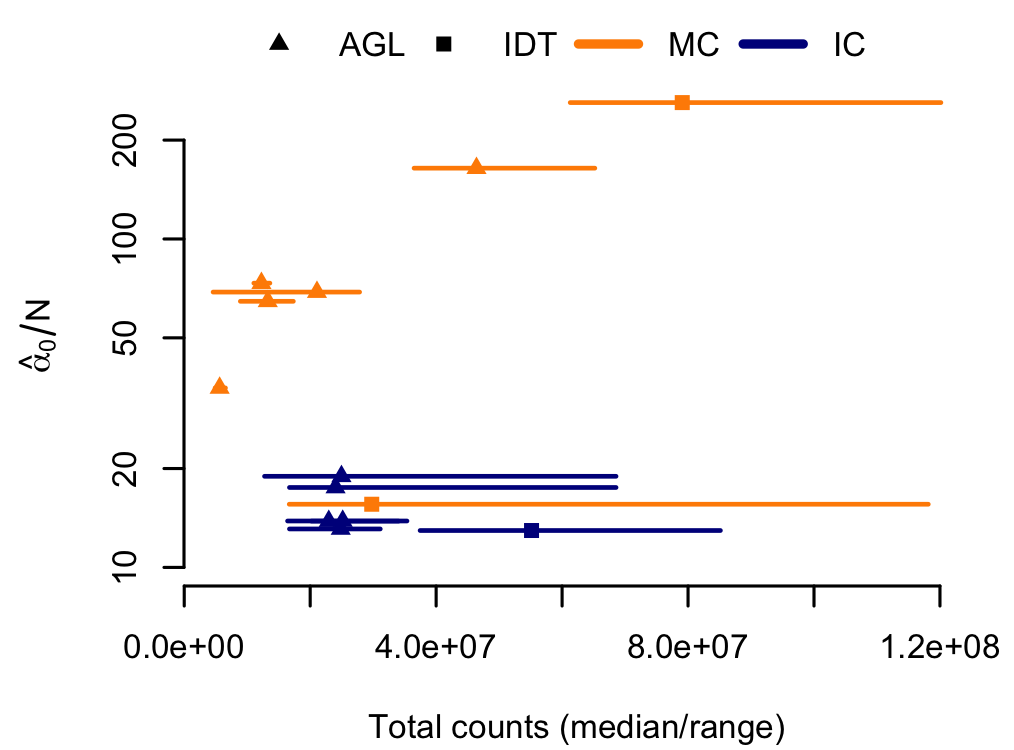
\includegraphics[]{figures-alpha0-1.pdf}
  \caption{Multiplexed capture (MC) decreases variance with respect to independent captures (IC), as estimated by fitting the dirichlet distribution. Total counts/sample given on the horizontal axis; mean $\alpha$ given on the vertical axis. $\alpha_0$ is inversely proportional to inter-sample variance. Each line/point represents a single pool. The point indicates the median total counts across the pool, with the range given by the line. Orange indicates a multiplexed capture; blue indicates independent captures. Triangles indicate pools using Agilent (AGL) capture; squares indicate Integrated DNA Technologies (IDT).}
  \label{fig:alpha0}
\end{figure}

The multiplexed pool without decreased inter-sample variance, IDT-MC, had a much larger spread in sequencing depth across the pool (\Cref{tab:poolSummary}, \Cref{fig:alpha0}).
Looking at the total mapped molecules, the IDT-MC pool had a relative standard deviation of 64.2\%, over double the next highest pool.
We hypothesized the absent reduction in variation stemmed from poor library balance during the multiplexing step.
We subsequently captured a new pool using the same DNA input, IDT-RR, and found comparable reductions in inter-sample variance (the pool with the highest $\alpha_0$ in \Cref{fig:alpha0}).

Examining the mean-variance relationship demonstrated the same inter-sample variance reduction suggested by the dirichlet parameter estimates (\Cref{fig:mnvr}).
The Agilent pools (\Cref{fig:mnvr}A) segregated cleanly, with less dispersion in the multiplexed capture pools.
Again, we found no variance reduction for the IDT-MC pool, overlapping with independently-captured IDT-IC pool (\Cref{fig:mnvr}B).
We did, however, observe near-complete reduction in dispersion for the better-balanced IDT-RR pool.

\begin{figure}
  \centering
  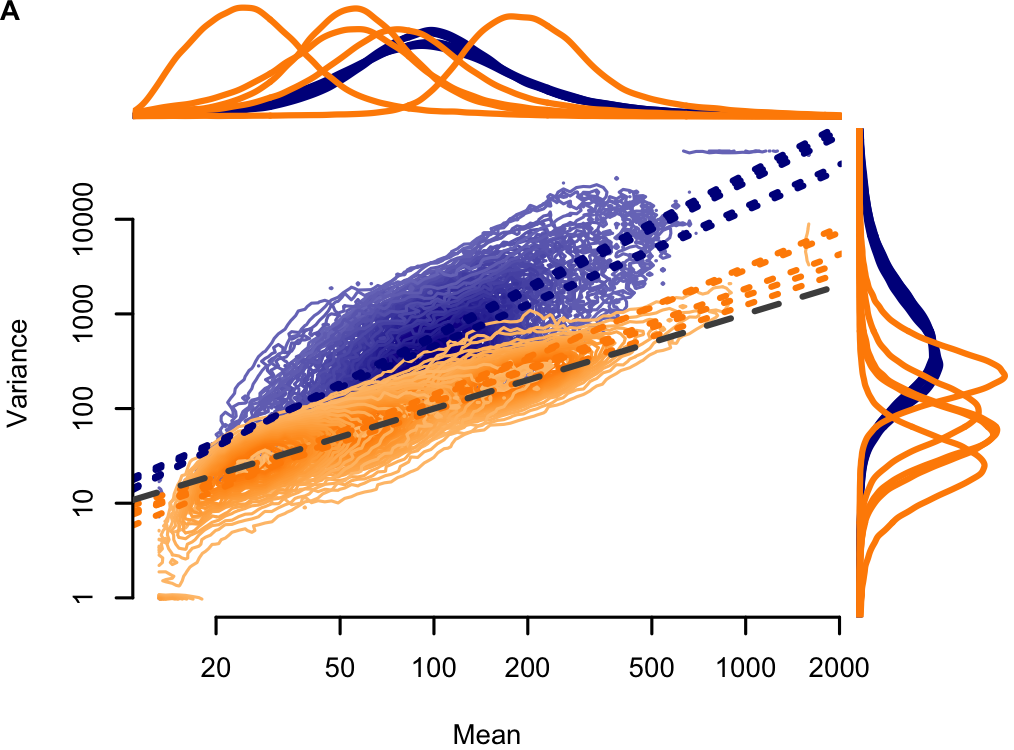
\includegraphics[]{figures-mnVrPlot-1.pdf}%
  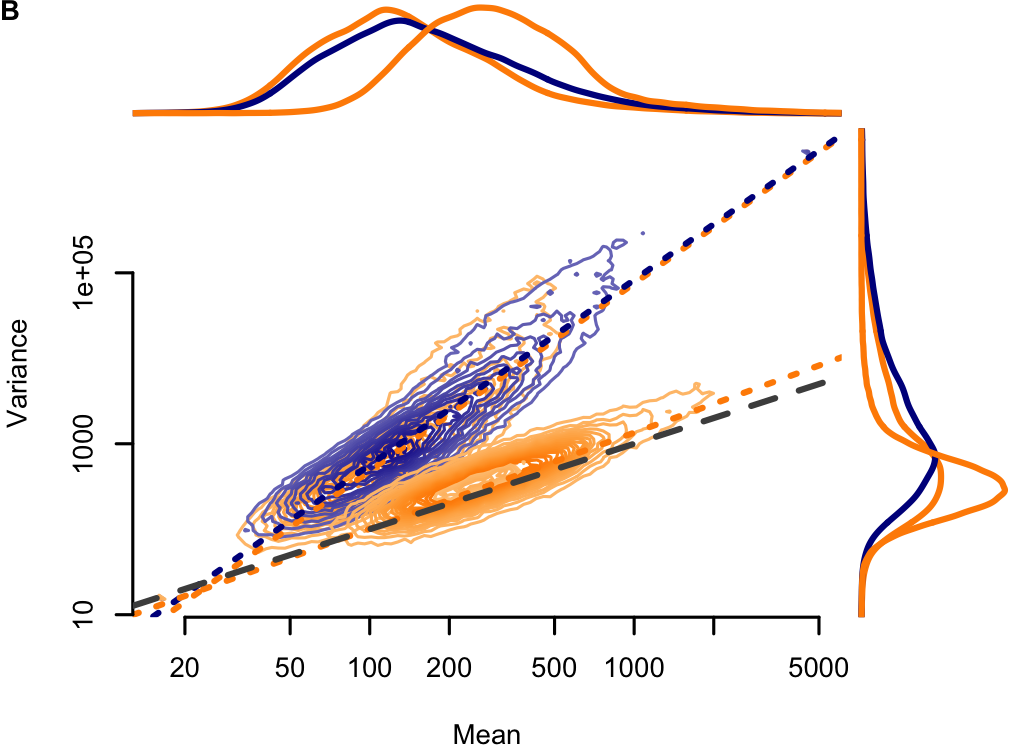
\includegraphics[]{figures-mnVrPlot-2.pdf}
  \caption{Mean-variance relationship demonstrates less dispersion in multiplexed capture. (A) Agilent (AGL) capture pools; (B) Integrated DNA Technologies (IDT) capture pools. Mean counts per exon given on the horizontal axis; mean variance per exon given on the vertical axis. Contours show the distribution of points by pool. Dotted lines show the ordinary least squares regression fit. Orange indicates multiplexed capture pools; blue indicates independently captured pools. The dashed gray line represents the 1:1 relationship expected under a Poisson process. Lines above the plot show the density of mean values by pool; lines to the right of the plot show the density of variance values by pool.}
  \label{fig:mnvr}
\end{figure}

\subsection{Multiplexed capture provides controls for ExomeDepth}

ExomeDepth requires a set of control subjects, summed into a reference vector of counts at each exon.
ExomeDepth provides functionality to select appropriate controls from a set of subjects, often requiring large numbers of subjects to identify appropriate controls.
Smaller research groups and clinical laboratories may struggle building large databases of exomes, with the difficulty compounded by lot-to-lot variation and regular improvements to capture and sequencing chemistries.
We wanted to know if the reduced inter-sample variance with multiplexed capture could provide an appropriate control set for ExomeDepth, eliminating the need for large databases of similarly-captured exomes.
We found the reduced inter-sample variance with multiplexed capture leads to appropriate control selection for ExomeDepth (\Cref{fig:edSelection}).
Pool2, where we repeated the initial fragmentation 5 times, did not perform as well as the other multiplexed pools.
We also found two samples within the WGS pool did not correlate well with the rest of the pool.

When we looked at independently-captured subjects, we found appropriate control sets for most of the 112 NCGENES subjects (\Cref{fig:edSelection}D).
However, ExomeDepth only selected 12.2\% of available samples as controls, on average (\Cref{fig:edSelection}C).
Similarly, with the independently-captured IDT-IC pool we find low control numbers for most samples.
While possible to select the same number of controls but exhibit differing dispersion, we observed little difference in the dispersion between independent and multiplexed capture (\Cref{fig:edSelection}B).
Overall, multiplexed capture provided appropriate controls for most samples tested, however an adequately-large set of available controls delivered comparable performance.

\begin{figure}
  \centering
  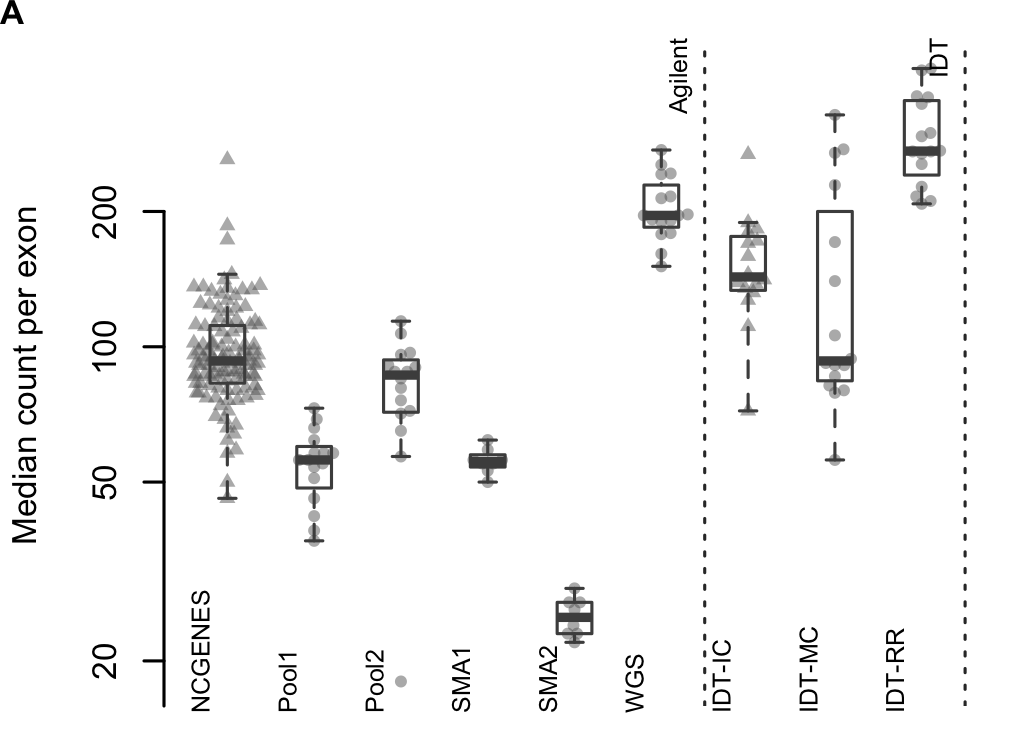
\includegraphics[]{figures-edSelection-1.pdf}%
  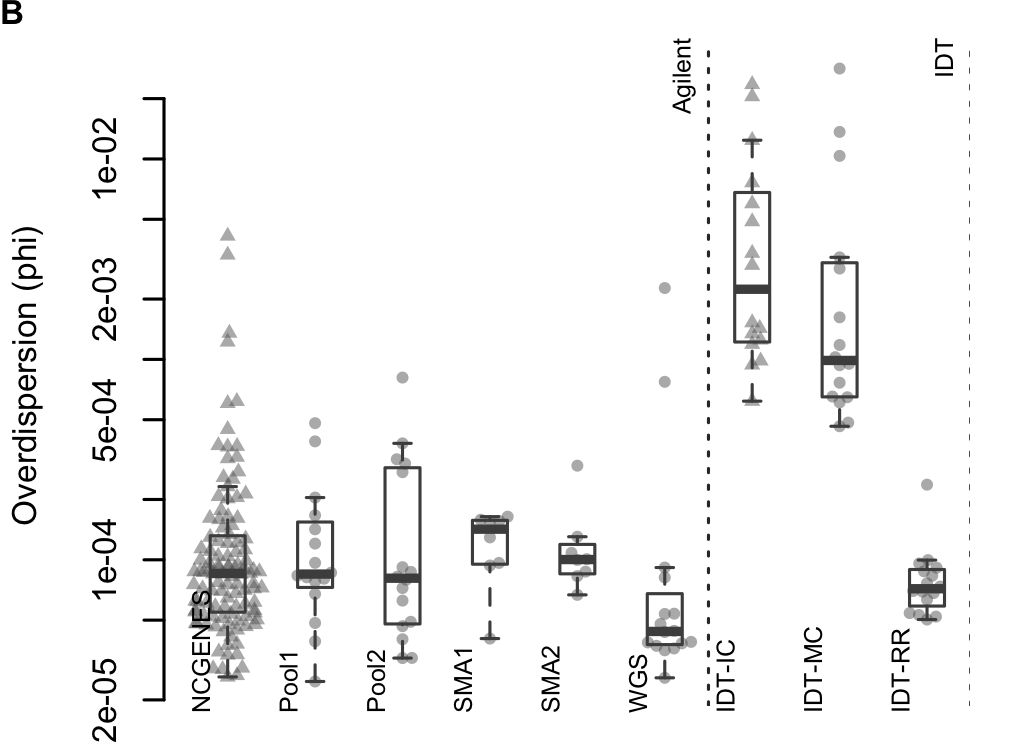
\includegraphics[]{figures-edSelection-2.pdf}
  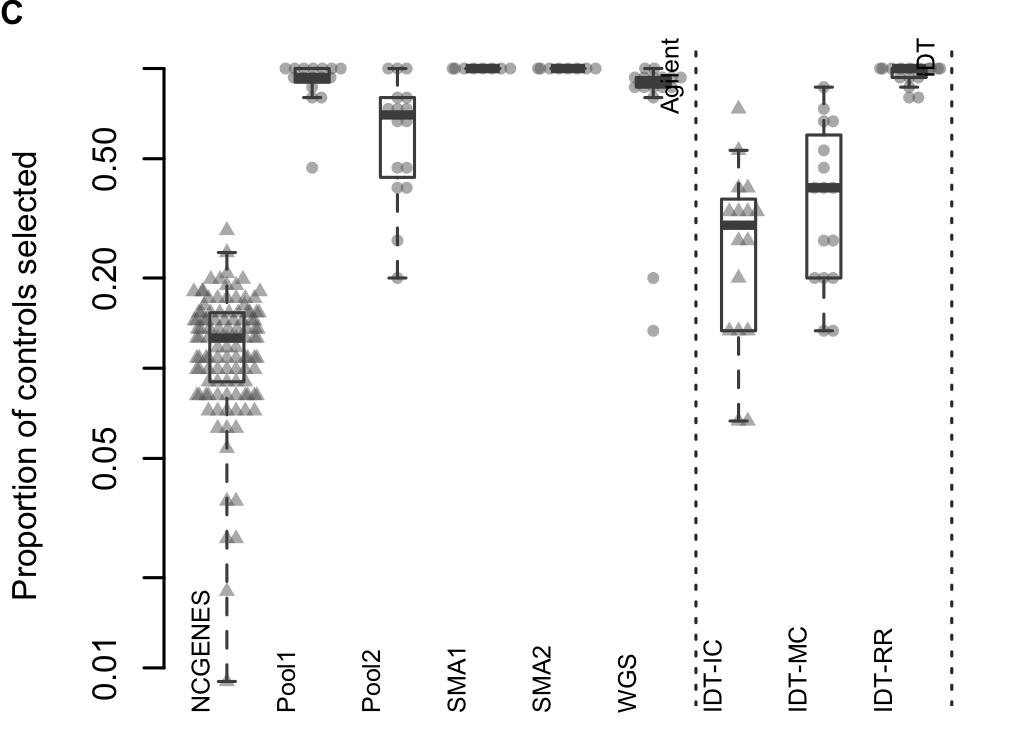
\includegraphics[]{figures-edSelection-3.pdf}%
  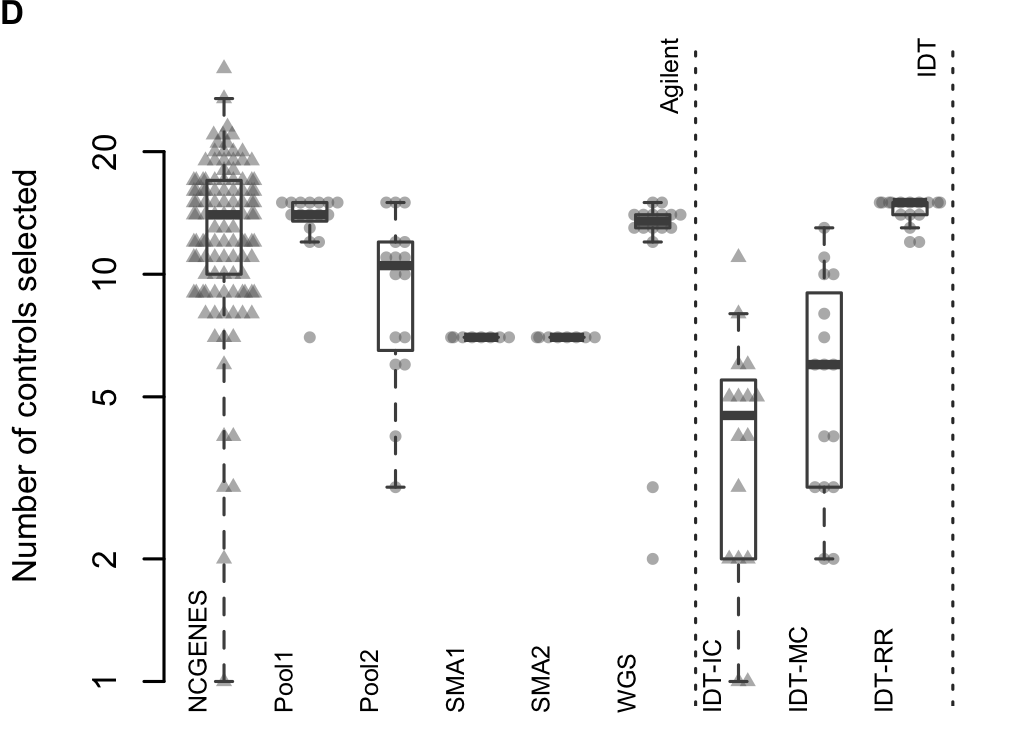
\includegraphics[]{figures-edSelection-4.pdf}
  \caption{ExomeDepth control selection. (A) median count per exon; (B) estimated phi parameter from ExomeDepth; (C) proportion of available samples selected as a control; (D) total number of controls selected. Each point represents a single sample, with samples grouped by pool. Triangles indicate independently-captured samples; circles indiciate a single multiplexed capture within the pool. Dotted vertical line separates the two capture platforms.}
  \label{fig:edSelection}
\end{figure}

\subsection{mcCNV \& ExomeDepth perform comparably in simulation study}

To compare our mcCNV algorithm and ExomeDepth, we created synthetic pools of data across different sequencing depths.
Based on our observations with the real data, we selected the total number of molecules for each sample from a uniform distribution defined as a 30\% window on either side of the specified depth; for example, for a specified depth of 10 million molecules, we drew the molecules per sample from 7 to 13 million molecules.
For each depth ranging from 5 to 100 million molecules, we simulated 200 16-sample pools with single-exon variants.
We allowed for homozygous and heterozygous deletions and duplications (0 to 4 copies), such that all variants were equally likely and the total variant probability was $1/1,000$.
We used, as the starting capture probabilities ($\mathbb{E}$), the empiric capture probabilities observed by summing across the Pool1 pool.

We analyzed each of the 4,000 pools (200 replicates by 20 depths) using our algorithm and two iterations of ExomeDepth.
For the first iteration of ExomeDepth, we used the default values for transition probability ($1/10,000$) and expected variant length (50 kb).
For the second iteration, we used the true simulated variant prior for the transition probability ($1/1,000$) and an expected variant length of 1 kb.
As expected, the sensitivity increased and false discovery rate decreased as the sequencing depth increased (\Cref{fig:simRes}).
In both comparisons, mcCNV demonstrated a superior false-discovery rate.
When interrogating Matthew's correlation coefficient \cite{matthews:1975aa} and the sensitivity, we found mcCNV had marginal performance over ExomeDepth with default parameters and marginal performance under ExomeDepth with simulation-matched parameters (table of values provided in supplemental materials).

\begin{figure}
  \centering
  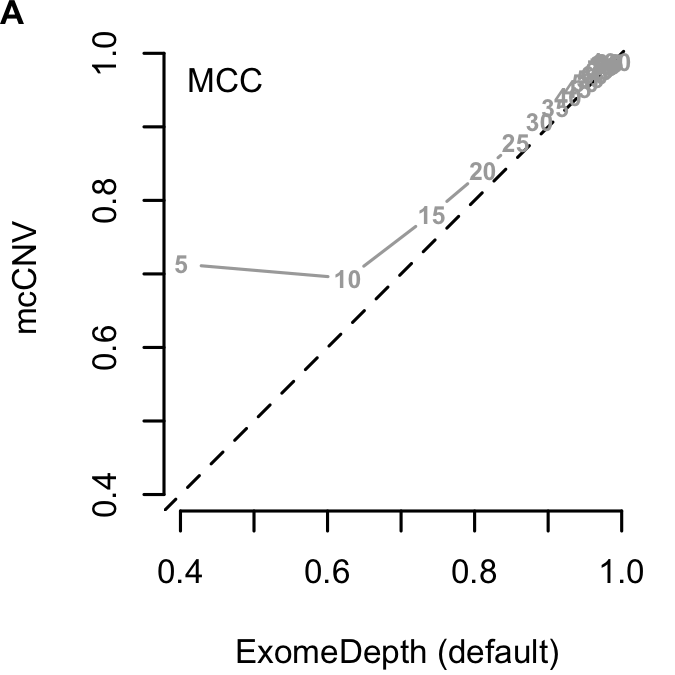
\includegraphics[]{figures-simPlts-1.pdf}%
  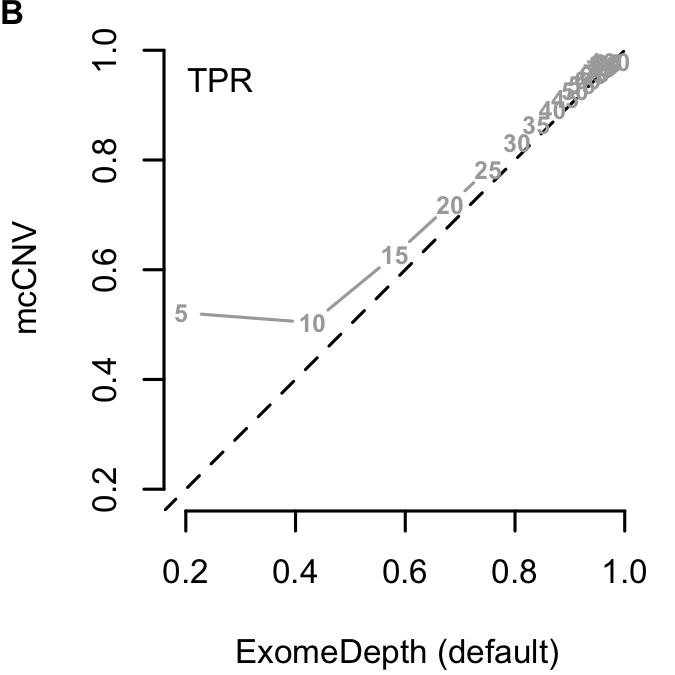
\includegraphics[]{figures-simPlts-2.pdf}%
  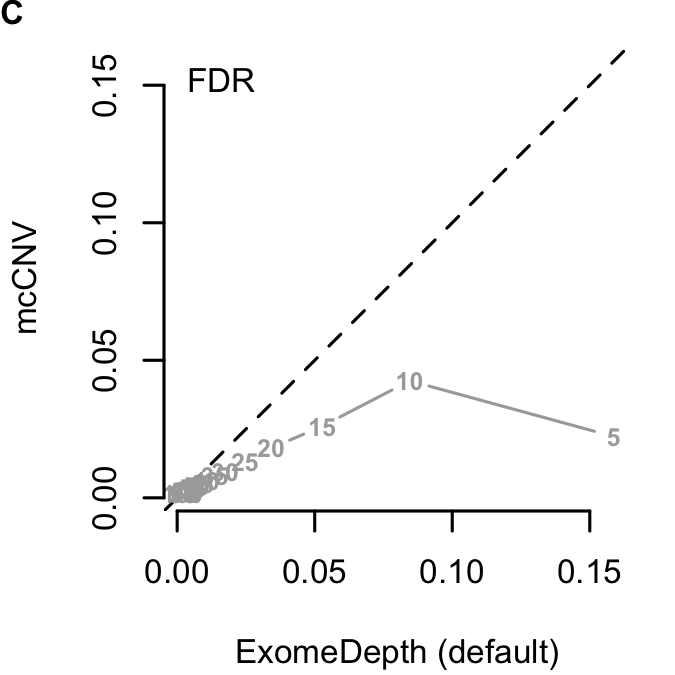
\includegraphics[]{figures-simPlts-3.pdf}
  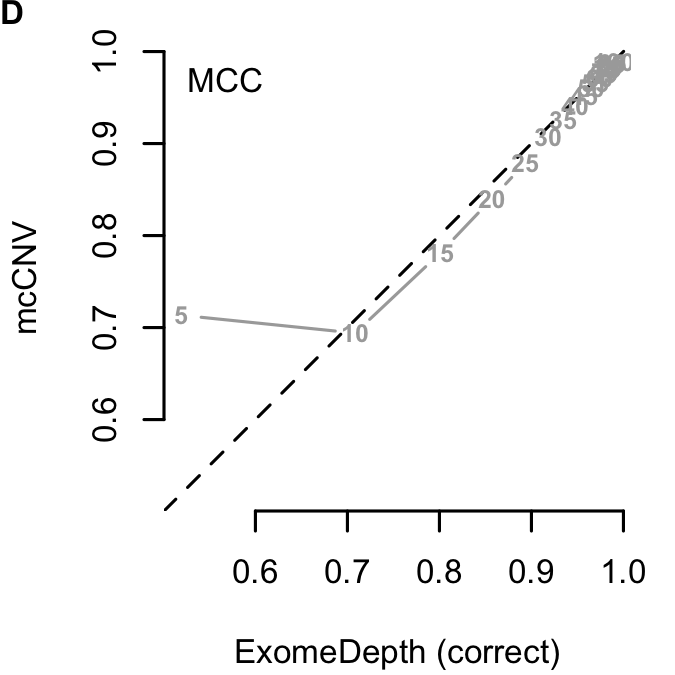
\includegraphics[]{figures-simPlts-4.pdf}%
  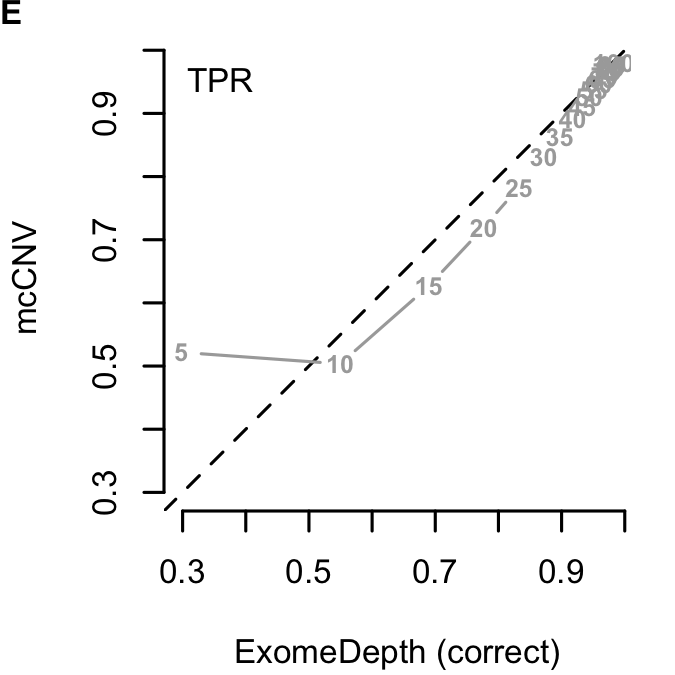
\includegraphics[]{figures-simPlts-5.pdf}%
  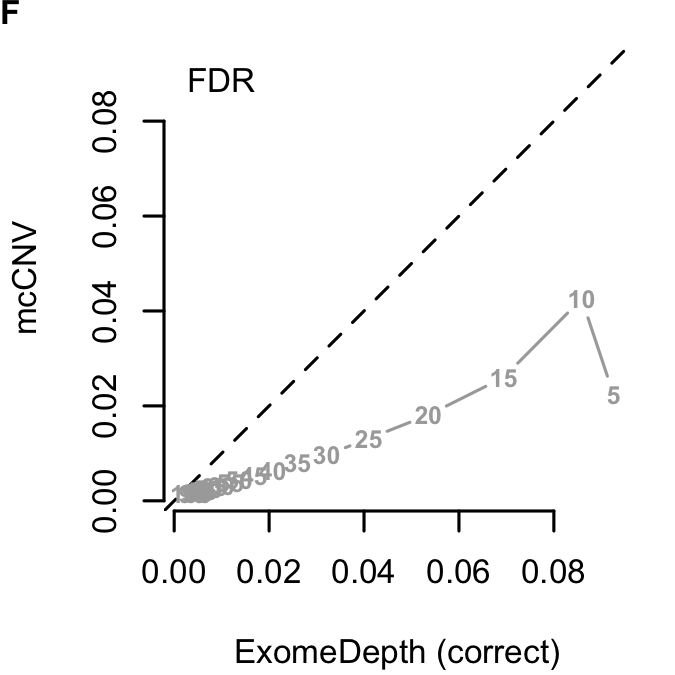
\includegraphics[]{figures-simPlts-6.pdf}
  \caption{Algorithm performance comparing mcCNV and ExomeDepth. (A-C) mcCNV versus ExomeDepth with default parameters, $1/10,000$ transition probability and 50 kb expected variant length. (D-F) mcCNV versus ExomeDepth with simulation-matched parameters, $1/1,000$ transition probability and 1 kb expected variant length. Numbered points indicate the simulated depth in millions of molecules. `MCC' indicates Matthew's correlation coefficient; `TPR' indicates true positive rate/sensitivity; `FDR' indicates false discovery rate. Dashed black line shows the 1:1 relationship.}
  \label{fig:simRes}
\end{figure}

\subsection{mcCNV \& ExomeDepth perform comparably on WGS pool}

To establish a truth set on real data, we performed matched genome sequencing on the subjects included in the WGS pool.
Following the best practices suggested by Trost et al. \cite{trost:2018aa}, we performed read-depth based CNV calling using the genome data.
In line with recommendations by Trost et al., we excluded from comparative  analysis any exons overlapping repetitive or low-complexity regions (34,856 out of 179,250).
We then compared the exome calls using mcCNV and ExomeDepth to the genome calls using the overlap of ERDS and cnvpytor.
\Cref{tab:wgsCallBySbj} lists the total calls by subject.
Overall, mcCNV predicted the largest number of variants; however, 85.7\% of predicted variants were deletions from two samples (NCG\_00790 and NCG\_00851).
ExomeDepth also predicted a disproportionate number of deletions for NCG\_00790 and NCG\_00851, totaling 69.4\% of calls.

% latex table generated in R 4.0.0 by xtable 1.8-4 package
% Mon Sep 14 15:35:24 2020
\begin{table}[]
\centering
\begin{tabular}{lrrrrrrrrr}
  \toprule   & \multicolumn{3}{c}{Total} & \multicolumn{3}{c}{Duplications} & \multicolumn{3}{c}{Deletions} \\ \cmidrule(lr){2-4}\cmidrule(lr){5-7}\cmidrule(lr){8-10}subject & MC & ED & WG & MC & ED & WG & MC & ED & WG \\ 
  \midrule
NCG\_00012 & 90 & 106 & 143 & 61 & 73 & 121 & 29 & 33 & 22 \\ 
  NCG\_00237 & 82 & 101 & 165 & 50 & 64 & 129 & 32 & 37 & 36 \\ 
  NCG\_00525 & 68 & 74 & 151 & 30 & 33 & 110 & 38 & 41 & 41 \\ 
  NCG\_00593 & 45 & 58 & 142 & 22 & 28 & 81 & 23 & 30 & 61 \\ 
  NCG\_00676 & 66 & 78 & 112 & 38 & 46 & 92 & 28 & 32 & 20 \\ 
  NCG\_00790 & 5156 & 2204 & 121 & 19 & 37 & 92 & 5137 & 2167 & 29 \\ 
  NCG\_00819 & 68 & 76 & 134 & 30 & 41 & 100 & 38 & 35 & 34 \\ 
  NCG\_00840 & 78 & 92 & 157 & 44 & 52 & 115 & 34 & 40 & 42 \\ 
  NCG\_00851 & 1151 & 859 & 141 & 28 & 51 & 102 & 1123 & 808 & 39 \\ 
  NCG\_00857 & 59 & 75 & 119 & 10 & 15 & 81 & 49 & 60 & 38 \\ 
  NCG\_00976 & 46 & 58 & 114 & 25 & 37 & 93 & 21 & 21 & 21 \\ 
  NCG\_01023 & 59 & 95 & 143 & 32 & 60 & 113 & 27 & 35 & 30 \\ 
  NCG\_01043 & 73 & 94 & 128 & 40 & 64 & 105 & 33 & 30 & 23 \\ 
  NCG\_01076 & 36 & 57 & 105 & 7 & 22 & 78 & 29 & 35 & 27 \\ 
  NCG\_01077 & 135 & 157 & 230 & 103 & 121 & 184 & 32 & 36 & 46 \\ 
  NCG\_01117 & 95 & 101 & 154 & 72 & 78 & 129 & 23 & 23 & 25 \\ 
   \bottomrule
\end{tabular}
\caption{Number of CNV calls by subject and algorithm for the `WGS' pool. `MC' indicates the mcCNV algorithm; `ED' indicates the ExomeDepth algorithm; `WG' indicates the overlap of ERDS/cnvpytor calls from matched whole-genome sequencing. Exons with any overlap of the repetitive and low-complexity regions, as defined in the Trost et al. manuscript, omitted from analysis.} 
\label{tab:wgsCallBySbj}
\end{table}


Looking at the control selection, for NCG\_00790 and NCG\_00851 ExomeDepth only selected 2 and 3 controls, respectively.
Furthermore, NCG\_00790 and NCG\_00851 had substantially higher dispersion than the rest of the pool (two outliers in \Cref{fig:edSelection}B).

Recognizing the genome calls do not represent an accurate truth set, we looked at the ability of mcCNV and ExomeDepth to predict the genome calls.
Due to the large number of deletions called for NCG\_00790 and NCG\_00851, both algorithms performed poorly in predicting the genome calls (\Cref{tab:predMetrics}).
When we excluded NCG\_00790 and NCG\_00851 from the analysis, mcCNV had comparable, but uniformly better performance.
Both algorithms demonstrated greater power to detect deletions.
\Cref{fig:wgsVenn} shows the call overlap, excluding NCG\_00790 and NCG\_00851, between the three approaches.

% latex table generated in R 4.0.0 by xtable 1.8-4 package
% Thu Oct  1 07:58:55 2020
\begin{table}[]
\centering
\begin{tabular}{cllrrrrr}
  \toprule
 &  &  & MCC & TPR & FDR & PPV & BalAcc \\ 
  \midrule
\cellcolor{white} &  & MC & 0.18 & 0.34 & 0.90 & 0.10 & 0.67 \\ 
  \cellcolor{white} & \multirow{-2}{*}{Full} & ED & 0.26 & 0.36 & 0.81 & 0.19 & 0.68 \\ 
   \rowcolor[gray]{0.9} \cellcolor{white} &  & MC & 0.49 & 0.34 & 0.31 & 0.69 & 0.67 \\ 
   \rowcolor[gray]{0.9} \multirow{-4}{*}{\cellcolor{white}\shortstack{DUP \\ + \\ DEL}} & \multirow{-2}{*}{Sub} & ED & 0.48 & 0.38 & 0.38 & 0.62 & 0.69 \\ 
   \midrule \cellcolor{white} &  & MC & 0.40 & 0.24 & 0.33 & 0.67 & 0.62 \\ 
  \cellcolor{white} & \multirow{-2}{*}{Full} & ED & 0.35 & 0.24 & 0.50 & 0.50 & 0.62 \\ 
   \rowcolor[gray]{0.9} \cellcolor{white} &  & MC & 0.40 & 0.25 & 0.33 & 0.67 & 0.62 \\ 
   \rowcolor[gray]{0.9} \multirow{-4}{*}{\cellcolor{white}DUP} & \multirow{-2}{*}{Sub} & ED & 0.38 & 0.27 & 0.45 & 0.55 & 0.63 \\ 
   \midrule \cellcolor{white} &  & MC & 0.18 & 0.64 & 0.95 & 0.05 & 0.82 \\ 
  \cellcolor{white} & \multirow{-2}{*}{Full} & ED & 0.22 & 0.56 & 0.91 & 0.09 & 0.78 \\ 
   \rowcolor[gray]{0.9} \cellcolor{white} &  & MC & 0.68 & 0.66 & 0.29 & 0.71 & 0.83 \\ 
   \rowcolor[gray]{0.9} \multirow{-4}{*}{\cellcolor{white}DEL} & \multirow{-2}{*}{Sub} & ED & 0.54 & 0.55 & 0.47 & 0.53 & 0.78 \\ 
   \bottomrule
\end{tabular}
\caption{mcCNV (MC)/ExomeDepth (ED) calls for `WGS' pool (used as prediction) versus the ERDS/cnvpytor calls from matched genome sequencing (used as truth). Calls are subdivided by duplications (DUP) and deletions (DEL). `Full' gives performance across the full pool; `Sub' gives the performance excluding the poorly correlated samples NCG\_00790 and NCG\_00851 (gray rows). `MCC' is Matthew's correlation coefficient, `TPR' is true positive rate/sensitivity, `FDR' is false discovery rate, `PPV' is positive predictive value, `BalAcc' is balanced accuracy. Exons with any overlap of the repetitive and low-complexity regions, as defined in the Trost et al. manuscript, omitted from analysis.} 
\label{tab:predMetrics}
\end{table}


\begin{figure}
  \centering
  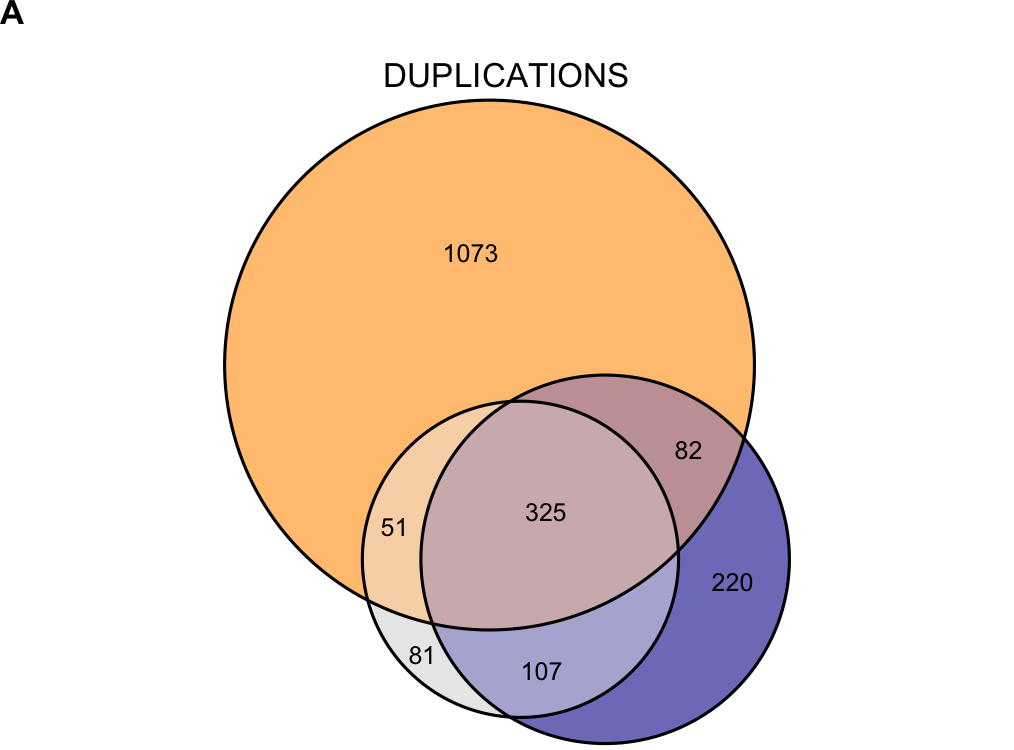
\includegraphics[]{figures-vennDiag-1.pdf}%
  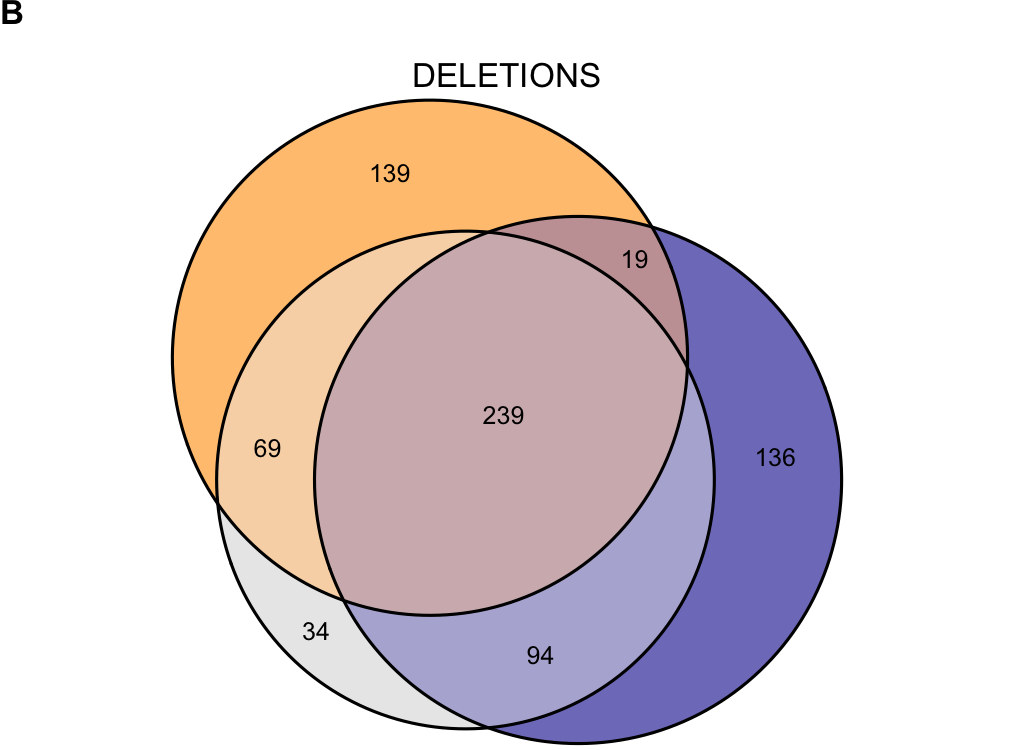
\includegraphics[]{figures-vennDiag-2.pdf}
  \caption{Copy number variant call concordance for the WGS pool, excluding subjects NCG\_00790 and NCG\_00851 due to poor correlation to the rest of the pool. (A) predicted duplications; (B) predicted deletions. mcCNV in grey; ExomeDepth in blue; ERDS/cnvpytor in orange. Values within overlaps give the number of variants.}
  \label{fig:wgsVenn}
\end{figure}


%%----------------------------------------------------------------------------%%
%% Discussion
%%----------------------------------------------------------------------------%%

\section{Discussion}

The medical genetics community still lacks robust exome-wide information about small (exon-level) variant prevalence.
Others have established the reliability and cost-efficiency of pre-capture multiplexing \cite{ramos:2012aa,wesolowska:2011aa,shearer:2012aa,neiman:2012aa,rohland:2012aa}, and most commercial exome capture platforms have protocols for pre-capture multiplexing.
Here, we demonstrate the reduction in inter-sample variance when pre-capture multiplexing, leading to increased power to detect exon-level copy number variation.
Despite the benefits, many clinical laboratories do not employ a multiplexed capture protocol because multiplexing requires waiting to fill a pool and may delay results.
While we understand the increased complexity, multiplexed capture may uncover otherwise missed copy number variation and increase the diagnostic yield for patients.

Multiplexed capture is not without limitations.
We presented an example (pool IDT-MC) where multiplexed capture provided little to no improvement over independently-captured samples.
We concluded the absent improvement in inter-sample variance stemmed from the poor library balance prior to capture.
Rebuilding a more-balanced pool with the same samples (pool IDT-RR) demonstrated a large reduction in inter-sample variance.

In assessing the inter-sample variance, we compared two capture platforms: (1) Agilent SureSelectXT2 and (2) Integrated DNA Technologies xGen Lockdown Probes.
We do not have enough data to suggest definitively one over the other.
Comparing the mean-variance relationship, the IDT-RR pool appeared to have less dispersion overall (supplemental materials); however, the sample-specific dispersion estimates from ExomeDepth suggest better performance by the WGS pool (\Cref{fig:edSelection}B) and the higher pool-wide dispersion comes entirely from the two poorly correlated samples.

Our results suggest having a sufficiently large database of samples most-often provides appropriate control samples to estimate copy number variation (\Cref{fig:edSelection}).
However, we show laboratories can circumvent the need for large samples by multiplexing the capture step.
Defining the capture pool as the set of controls both limits the need for regular reanalysis as the database grows and eliminates potential over-selecting of samples with the same variants.

At the depth of the WGS pool, our simplistic simulation study would suggest both mcCNV and ExomeDepth have the power to detect single-exon variants with $>$85\% sensitivity while maintaining a low false-discovery rate (\Cref{fig:simRes}, supplemental materials).
However, comparing the exome calls to the genome calls for the WGS pool revealed lackluster concordance.
As Trost et al. point out, the genome CNV callers still struggle with variants less than 1 kb \cite{trost:2018aa}.
We do not dismiss the possibility of exome calls providing greater reliability than the genome calls, given multiplexed capture and adequate sequencing depth.
However, given the distribution of calls throughout the exome, we doubt the thousands of excess deletions called for NCG\_00790 and NCG\_00851.
Confirmation of the individual calls is beyond the scope of this work.

Unsurprisingly, both mcCNV and ExomeDepth failed to call many of the duplications called from the genome data.
The variance for the negative binomial increases as the mean increases; we expect greater variation in read depth from duplicated loci, making duplications more difficult to distinguish.
Similarly, the variance of the binomial proportion increases monotonically over [0, 0.5).
More sensitive detection of duplications will likely require greater sequencing depth.

The simulation study emphasizes the importance of sequencing depth (in terms of absolute molecules).
We can collect increased basepair coverage for less money by sequencing longer reads (e.g. 2x150 versus 2x50), but doing so decreases power for depth-based CNV calling.
Typically, exome sequencing targets 30-50x coverage to ensure most targets have sufficient coverage for accurate basepair calling.
We demonstrate the need for much deeper sequencing if we wish to establish exon-level variants.

Taken together, we recommend the following:
(1) research and clinical endeavors consider adjusting protocols to multiplex samples prior to any targeted capture;
(2) prior to capture, we suggest checking the library balance and adjusting as necessary (we achieved reasonable performance with relative standard deviation values less than 25\%);
(3) collecting an average of 225 filtered read-pairs per target.
We then provide a simple-to-use and efficient R package to estimate copy number utilizing the negative bionimal distribution.

We believe the uncertainty about the prevalence and clinical significance of exon-level variants warrants a large undertaking.
Even if we take the conservative approach and looking only at concordant calls between genome and exome sequencing (Figure 5), we have an average of 40 variants per sample to contend with.
Two possibilities exist: (1) the algorithms all fail over specific regions, or (2) some genes can tolerate intrageneic copy-number variation better than others.
Having eliminated calls from repetitive and low-complexity regions, we believe possibility (2) is more likely.
To truly determine the prevalence (and therefore, clinical significance) of exon-level variants we need to interrogate exon-level variants on a large cohort.
Confirmation testing for the tens to thousands of predicted variants from the exome and genome calls would allow true determination of algorithm performance and inform the clinical utility.

\section{Funding information}

This work was supported by the National Institute of Child and Human Development [F30HD101228] and by the National Institute of General Medical Sciences [5T32GM067553].

%%----------------------------------------------------------------------------%%
%% References
%%----------------------------------------------------------------------------%%

\bibliographystyle{plain}
\bibliography{/Users/dayne/Github/mybibs/myBib}

\end{document}
